% ****** Start of file apssamp.tex ******
%
%   This file is part of the APS files in the REVTeX 4.2 distribution.
%   Version 4.2a of REVTeX, December 2014
%
%   Copyright (c) 2014 The American Physical Society.
%
%   See the REVTeX 4 README file for restrictions and more information.
%
% TeX'ing this file requires that you have AMS-LaTeX 2.0 installed
% as well as the rest of the prerequisites for REVTeX 4.2
%
% See the REVTeX 4 README file
% It also requires running BibTeX. The commands are as follows:
%
%  1)  latex apssamp.tex
%  2)  bibtex apssamp
%  3)  latex apssamp.tex
%  4)  latex apssamp.tex
%
\documentclass[%
 reprint,
superscriptaddress,
%groupedaddress,
%unsortedaddress,
%runinaddress,
%frontmatterverbose, 
%preprint,
%preprintnumbers,
%nofootinbib,
%nobibnotes,
%bibnotes,
 amsmath,amssymb,mathtools,
%aps,
pre,
%prb,
%rmp,
%prstab,
%prstper,
floatfix,
]{revtex4-2}

\usepackage{graphicx}% Include figure files
\usepackage{dcolumn}% Align table columns on decimal point
\usepackage{bm}% bold math
\usepackage{hyperref}% add hypertext capabilities
\usepackage{mathtools}
\usepackage{tikz}
\usepackage{physics}
\usepackage{placeins}
\usepackage{dsfont}
\usepackage{ifthen}
\usepackage{enumitem} 
%\usepackage[mathlines]{lineno}% Enable numbering of text and display math
%\linenumbers\relax % Commence numbering lines

%\usepackage[showframe,%Uncomment any one of the following lines to test 
%%scale=0.7, marginratio={1:1, 2:3}, ignoreall,% default settings
%%text={7in,10in},centering,
%%margin=1.5in,
%%total={6.5in,8.75in}, top=1.2in, left=0.9in, includefoot,
%%height=10in,a5paper,hmargin={3cm,0.8in},
%]{geometry}

\newcommand{\hbarE}{{\hbar_{\text{eff}}}}
\newcommand{\te}[1]{\text{#1}}
\newcommand{\tLoc}{\ensuremath{\tau_{\rm s}}}
\newcommand{\tLeak}{\ensuremath{\tau_{\rm L}}}
\newcommand{\tEhr}{\ensuremath{\tau_{\rm E}}}

\newcommand{\ha}[1]{\ensuremath{\hat{a}_{#1}}}
\newcommand{\had}[1]{\ensuremath{\hat{a}^{\dagger}_{#1}}}
\newcommand{\rc}[1]{{\color{red} #1}}
\newcommand{\ls}{\ensuremath{\lambda_{\rm s}}}
\newcommand{\lL}{\ensuremath{\lambda_{\rm L}}}
\renewcommand{\lq}{\ensuremath{\lambda_{\rm q}}}
\renewcommand{\d}{\ensuremath{\operatorname{d}\!}}
%\bibliographystyle{apsrev4-2.bst}
\bibliographystyle{aipnum4-2.bst}
\setcitestyle{numbers,square,sort&compress}

\begin{document}

\preprint{PRE }

\title{A dynamical transition from localized to uniform scrambling \\ in locally hyperbolic systems}% Force line breaks with \\
%\thanks{A footnote to the article title}%

\author{Mathias Steinhuber} %\email{mathias.steinhuber@ur.de}
\affiliation{%
 Institut f\"ur  Theoretische Physik, Universit\"at Regensburg, 
  93040 Regensburg, 
 Germany
 }
\author{Peter Schlagheck} %\email{peter.schlagheck@uliege.be}
\affiliation{%
 CESAM Research Unit, University of Liege, 4000 Liège, Belgium
}

\author{Juan Diego Urbina}%
 \affiliation{%
 Institut f\"ur  Theoretische Physik, Universit\"at Regensburg, 
 93040 Regensburg, 
 Germany
 }
\author{Klaus Richter}%
\affiliation{%
 Institut f\"ur  Theoretische Physik, Universit\"at Regensburg,
  93040 Regensburg, 
 Germany
}

\date{\today}% It is always \today, today,
             %  but any date may be explicitly specified

\begin{abstract}
Fast scrambling of quantum correlations, reflected by the exponential growth of Out-of-Time-Order Correlators (OTOCs) on short pre-Ehrenfest time scales, is commonly considered as a major signature of quantum chaos in quantum systems with a classical limit. In two recent works, by Hummel et al.~\cite{Hummel2019} and by Scaffidi et al.~\cite{Scaffidi2020}, a significant difference in the  scrambling rate of integrable (many-body) systems was observed, depending on the initial state being semiclassically localized around unstable fixed points or fully delocalized (infinite temperature). Specifically, the quantum Lyapunov exponent $\lq$ quantifying the OTOC growth is given, respectively, by $\lq=2\ls$ or $\lambda_{\rm q}=\ls$ in terms of the stability exponent $\ls$ of the hyperbolic fixed point. Here we show that a wave packet, initially localized around this fixed point, features a distinct {\it dynamical} transition between these two regions. We present an analytical semiclassical approach providing a physical picture of this phenomenon and support our findings by extensive numerical simulations in the whole parameter range of locally unstable dynamics of a Bose-Hubbard dimer. Our results suggest that the existence of this transition is a hallmark of unstable separatrix dynamics in integrable systems. This allows one to distinguish, within the exponential OTOC growth behavior, unstable integrable (many-body) dynamics from genuine chaotic dynamics featuring uniform growth.

% A major signature of quantum chaos is the fast scrambling of quantum correlations, reflected by the quantum Lyapunov exponent $\lq$ that quantifies the short-(pre-Ehrenfest) time exponential growth of Out-of-Time-Order Correlators (OTOCs) in systems displaying unstable classical dynamics. In two recent works, by Hummel et al. and by Scaffidi et al., it was observed that around unstable fixed points of integrable systems there is a significant difference in the rate of scrambling depending on the nature of the initial state being quasiclassically localized or fully delocalized (infinite temperature). Specifically, the quantum Lyapunov exponent is given respectively by $\lq=2\ls$ or $\lambda_{\rm q}=\ls$ in terms of the stability exponent $\ls$ of the hyperbolic fixed point. We show here that a quasiclassical wave-packet localized around the fixed point displays in fact a clear {\it dynamical} transition between these two regions and, by extending previous quasiclassical analysis into the time domain, we present an analytical approach providing a physical picture of this phenomenon. Our findings, supported by extensive numerical simulations in all the range of parameters where a system of interacting bosons in two wells displays locally unstable dynamics, suggest that the existence of the transition is a hallmark of separatrix dynamics in integrable systems and therefore allows to use its absence in the OTOCs  as a signature of  genuine chaos. 
\end{abstract}
\maketitle
%\keywords{Integrable Dynamics, Separatrix Motion, Out-of-Time-Order Correlator, Scrambling}
\section{Introduction}

The increasing complexity of source code poses a key challenge to the reliability of large-scale software systems. Software bugs in these systems can lead to safety issues~\cite{bug_safety} for users around the world as well as cause non-negligible financial losses~\cite{bug_loss}. As such, developers have to spend a large amount of time and effort on bug fixing. Consequently, \aprfull (\apr), designed to automatically generate patches to fix software bugs, has attracted wide attention from both academia and industry~\cite{long2016prophet, legoues2012genprog, long2015spr, lou2020can, tufano2018empstudy}. 


To achieve \apr, one popular approach is known as Generate-and-Validate (G\&V)~\cite{qi2015gv, ghanbari2019prapr, lou2020can, le2016hdrepair, legoues2012genprog, wen2018capgen, hua2018sketchfix, martinez2016astor, koyuncu2020fixminder, liu2019tbar, liu2019avatar}, which is typically based on the following pipeline: First, fault localization techniques~\cite{wong2016fl, abreu2007ochiai, zhang2013injecting, papadakis2015metallaxis, li2019deepfl, li2017transforming} are applied to determine the suspicious locations in programs where bugs are likely to exist. Then, the buggy locations are used by the \apr tools to generate a list of patches that replace buggy lines with correct lines. Afterward, each patch is validated against the original test suite to identify any \emph{plausible patches} (i.e., passing all tests in the test suite). Finally, to determine the \emph{correct patches}, developers examine the list of plausible patches to see if any of them can correctly fix the bug. 

Traditional \apr tools can mainly be categorized into heuristic-based~\cite{legoues2012genprog, le2016hdrepair, wen2018capgen}, constraint-based~\cite{mechtaev2016angelix, le2017s3, demacro2014nopol, long2015spr} and \template~\cite{ghanbari2019prapr, hua2018sketchfix, martinez2016astor, liu2019tbar, liu2019avatar}. Among these traditional tools, \template \apr tools~\cite{ghanbari2019prapr, liu2019tbar, benton2020effectiveness} have been able to achieve state-of-the-art results. \Template \apr tools typically leverage pre-defined templates (e.g., adding a nullness check) for bug fixing. However, since these fix templates are typically handcrafted, the number and types of bugs they are able to fix can be limited. 



To address the limitations of traditional \apr, researchers have proposed various \learning \apr tools~\cite{li2020dlfix, chen2018sequencer, jiang2021cure, lutellier2020coconut, zhu2021recoder, ye2022rewardrepair} based on the \nmtfull (\nmt) architecture~\cite{sutskever2014mt} where the input is the buggy code snippets and the goal is to translate the buggy code snippets into a fixed version. To accomplish this, \learning \apr tools require supervised training datasets with pairs of both buggy and fixed code snippets in order to learn how to perform this translation step. These training data are usually obtained by mining historical bug fixes using heuristics/keywords~\cite{dallmeier2007benchmark}, which can be imprecise for identifying bug-fixing commits; even the actual bug-fixing commits can include irrelevant code changes, leading to further pollution in the dataset~\cite{xia2022alpharepair}.
% 
Moreover, it can be hard for such \apr tools to generalize and fix bug types unseen during training. 



To better leverage recent advances in \plmfull{s} (\plm{s}), researchers~\cite{xia2022alpharepair, xia2023repairstudy, kolak2022patch, prenner2021codexws} have directly applied \plm{s} to generate patches without bug-fixing datasets. These \llm-based \apr tools work by either directly generating a complete code function~\cite{prenner2021codexws, xia2023repairstudy} or predict/infill the correct code snippet given its surrounding context~\cite{xia2022alpharepair, xia2023repairstudy}. By directly using \llm{s} that are pre-trained on billions of open-source code snippets, \llm-based \apr tools can achieve state-of-the-art performance on many repair datasets~\cite{xia2022alpharepair}. 


% 
%
%

Traditional \apr tools have long used the insight of the \emph{plastic surgery hypothesis}~\cite{barr2014plastic} where it states that the code ingredients to fix a bug already exist within the same project. Traditional \apr tools have manually designed pattern-~\cite{ghanbari2019prapr, saha2017elixir} or heuristic-based~\cite{jiang2018simfix, legoues2012genprog} approaches to finding and using such relevant code ingredients to generate fixes for bugs. However, the plastic surgery hypothesis has been largely ignored in \llm-based \apr. In fact, \llm provides a unique opportunity to fully automate the plastic surgery hypothesis idea via fine-tuning (learning project-specific information via model updates from the buggy project) and prompting (directly providing relevant code ingredients to the model), and make it directly applicable to different languages (since the \llm{s} are typically multi-lingual).%
Moreover, despite the intensive manual efforts involved, traditional \apr tools still cannot fully leverage project-specific information due to large search space for leveraging/composing existing code ingredients. In contrast, the project-specific information can effectively leveraged by \llm{s} due to their power in code understanding/vectorization, e.g., even partial/imprecise information may still guide \llm{s} in correct patch generation!
 To this end, we ask the question: \emph{How useful is the plastic surgery hypothesis in the era of \plm{s}}?








\mypara{Our Work.} To answer the question, we present \ourtech{\xspace} -- a \llm-based approach that automatically utilizes the plastic surgery hypothesis by systematically combining multiple fine-tuning and prompting strategies for \apr. \ourtech fine-tunes \plm{s} using two novel domain-specific training strategies: \textbf{\epfinetune} -- we fine-tune using the original buggy project by aggressively masking out a high percentage of tokens, which allows \plm to learn project-specific code tokens and programming styles; and \textbf{\rofinetune} -- which only masks out a single continuous code sequence per training sample, allowing the model to get used to the final \csapr task of predicting a single continuous code sequence. Furthermore, we directly leverage the ability for \plm{s} to understand natural language instructions and introduce a novel prompting strategy, \textbf{\idprompting}, which uses information retrieval and static analysis to obtain a list of relevant identifiers for the buggy lines. While such relevant identifiers are critical for fixing some difficult bugs, they may not be seen by the \llm during inference due to limited context window size. Through the use of prompting, we directly tell the model to use these extracted identifiers (relevant code ingredients) to generate the correct code. Finally, to perform repair, we combine all four model variants (including the base model, both fine-tuned models and the base model with prompting) for the final repair.





While our insight of leveraging the plastic surgery hypothesis for \llm-based \apr is generalizable across different types of \plm{s}, to implement \ourtech, we choose a recent \plm{\xspace}, \ctfive~\cite{wang2021codet5}, which is pre-trained on millions of open-source code snippets. \ctfive is an encoder-decoder model trained using \mspfull (\msp) objective where a percentage of tokens are masked out and each continuous masked token sequence is referred to as a masked span. Also, although we only extract relevant identifiers from the current buggy project (since this paper focuses on the plastic surgery hypothesis), our work can be easily extended to obtain other code information (such as relevant statements or functions) from other sources, such as  the massive pre-training corpora~\cite{husain2020codesearchnet} or historical bug-fixing datasets~\cite{jiang2019infer}, which can provide more coding knowledge for \llm{s}. Besides, although we mainly focus on using traditional string comparison algorithms for information retrieval in this paper, these techniques can be easily replaced by other frequency-based retrieval~\cite{robertson2009probabilistic} and neural search (or embedding-based search)~\cite{reimers2019sentence}.
  In summary, this paper makes the following contributions:


%


\begin{itemize}[noitemsep, leftmargin=*, topsep=0pt]
    \item \textbf{Dimension.} This paper is the first to revisit the important plastic surgery hypothesis in the era of \llm{s}. It opens up a new dimension for \llm-based \apr to incorporate previously neglected information from the buggy project itself to boost \apr performance. Furthermore, it demonstrates the promising future of retrieval-based prompting for modern \llm-based \apr.
    \item \textbf{Implementation.} We implement \ourtech based on the recent \ctfive model. We augment the model using two novel fine-tuning strategies: \epfinetune and \rofinetune, along with a novel prompting strategy based on information retrieval and static analysis: \idprompting. We combine the patches generated by all four models together and perform patch ranking to speed up \apr.% 
    \item \textbf{Evaluation Study.} We conduct an extensive evaluation against state-of-the-art \apr tools. On the widely studied \dfj 1.2 and 2.0 datasets~\cite{just2014dfj}, \ourtech is able to achieve the new state-of-the-art results of 89 and 44 correct bug fixes (15 and 8 more than best baseline) respectively.  Furthermore, we perform a broad ablation study to justify our design. \ourtech demonstrates for the first time that the plastic surgery hypothesis can substantially boost \llm-based \apr and advance state-of-the-art \apr, while being fully automated and general. Moreover, even partial/imprecise code ingredients may still effectively guide \llm{s} for \apr!
\end{itemize}



\section{Out-of-Time-Order Correlator in~integrable~systems with local hyperbolicity}%
\label{sec:OTOC_theory}%
Our goal in this section is to refine the pre-Ehrenfest theory for scrambling around hyperbolic fixed points in integrable systems. In particular we attempt to relax the localization properties of the initial state considered in~\cite{Hummel2019,Scaffidi2020}.
%
The OTOC for two operators $\hat{A}$, $\hat{B}$ with respect to a state $\hat{\rho}$ is defined by 
\begin{align}
    \mathbf{ C}(t) \,=\, \operatorname{tr} \big\{\hat{\rho} \big| [\hat{A}(t),\hat{B} ] \big|^2 \big\},
    \label{eq:OTOC_def} 
\end{align}
which is by itself a modulus-squared commutator. When this squared commutator is expanded in individual correlators one obtains, besides contributions that admit a standard time ordering, extra irreducibly un-ordered correlations \cite{Maldacena_2016}, with anomalous dynamical behavior that are the central object of study.  

The long-time~(post-Ehrenfest) saturation of generic OTOCs has been subject of several studies, both in the chaotic \cite{Josef2018,argentinians} and integrable \cite{Hummel2019,Fortes} regimes where interference effects beyond a pure quasiclassical (Truncated-Wigner like-) approach appear~\cite{Polkovnikov2011}.

Here, however, our focus is the short time scales, where a quasiclassical approach based on the Wigner-Moyal expansion, which is a regular expansion around $\hbarE=0$ \cite{schleich01,Kim1991,connell2008}, is perfectly appropriate. Keeping only leading-order terms in $\hbarE$, one obtains %(see App.~\ref{sec:appendixWignerMoyal})\rc{maybe an appendix? YES but not in present arXiv version, just put as reference the quantum optics in phase space book}

    \begin{align}
        \begin{split}
            \mathbf{ C}(t) \,=\,& \hbarE^{2} \langle W_{\rho}(\Vec{q}_{0},\Vec{p}_{0}) \big|\big\{ A_{\rm W}(\Vec{q}_{0},\Vec{p}_{0},t), B_{\rm W}(\Vec{q}_{0},\Vec{p}_{0}) \big\}  \big|^{2}\rangle_{\text{PS}}
            \\
            &+ O(\hbarE^{4}),
        \end{split}
         \label{eq:WignerWeyl}
    \end{align}
    where $A_{W}$, $B_{W}$ are the Wigner-transforms of the operators $\hat{A},\hat{B}$ and $W_{\rho}(\Vec{q}_{0},\Vec{p}_{0})$   is the Wigner-distribution corresponding to the state $\hat{\rho}$. 

    
    Further, $\langle  . \rangle_{\text{PS}}$ indicates integration over the whole classical (mean-field) phase space parametrized by the canonical pairs $(\Vec{q}_{0},\Vec{p}_{0})$. The Heisenberg time dynamics of the quantum operator is mapped to time dynamics of the classical observable $A(q_{0},p_{0},t) =A(q(q_{0},p_{0},t),p(q_{0},p_{0},t)) $ which arises from the classical propagation of the initial values $q_{0}$ and $p_{0}$.
    
    The effective Plank constant $\hbarE$ has different expressions in different contexts. It is given by the usual Plank constant divided a typical action $\hbar/S_{\rm typ}$ in single particle cases \cite{Gutzwiller1991,Haake2001,brack1997}, and the inverse of the total spin quantum number $1/S$ for spin systems \cite{Waltner2017PRL,Waltner2020PRE}. In the case of interest here, interacting bosonic systems, $\hbarE = \frac{1}{N}$  is given by the inverse of the total particle number $N$ after convenient rescaling of the interaction strength \cite{Richter2022,Engl2015PRE}.
    
    Without loss of generality, we choose the operators $\hat{A}=\hat{q}$ and $\hat{B}=\hat{p}$, as they are hermitian and their classical counterparts are generalized coordinates or momenta. Therefore, at leading order in the Wigner-Moyal expansion, Eq.~\eqref{eq:WignerWeyl},
    we drop the index ${}_W$ and take the pure classical phase space functions. This choice of the operators simplifies the classical Poisson-brackets, that are now given by an element of the stability matrix $\frac{\partial \vec{x}(t)}{\partial \vec{x}(0)}$ with $\vec{x} = (\vec{q},\vec{p})$ \cite{tabor1989chaos,wiggins2003}. 

    The classical limit of the OTOC in Eq.~(\ref{eq:WignerWeyl}) is so far a completely general result. Under the assumption of local instability, however, the leading order of exponential growth is given by the maximal local exponent $\lambda(\vec{q}_{0},\vec{p}_{0})$ of the stability matrix:
    \begin{align}
         \mathbf{ C}(t) ~\sim~& \hbarE^{2} \langle W_{\rho}(\Vec{q}_{0},\Vec{p}_{0}) \exp\big\{ 2 \lambda(\Vec{q}_{0},\Vec{p}_{0}) t\big\}  \rangle_{\text{PS}}.
         \label{eq:WignerWeylFP}
    \end{align}
    
    At this point, it is convenient to introduce two local time-scales:
    \begin{itemize}
        \item After the local ergodic time $\tLoc= 1/\lambda (\Vec{q}_{0},\Vec{p}_{0})$,  the exponential growth of the OTOC begins to be visible. Before $\tLoc$, we have sub-exponential/polynomial behavior linked to system-specific mechanisms.
        \item The Wigner-Weyl approximation breaks down when the leading order of the integrand in Eq.~\eqref{eq:WignerWeyl} becomes large compared to $\hbarE^{2}$. This breakdown defines the local Ehrenfest time $\tEhr= \lambda^{-1}(\Vec{q}_{0},\Vec{p}_{0})  \log (1/\hbarE)$ and in our many-body case $\tEhr= \lambda^{-1}(\Vec{q}_{0},\Vec{p}_{0}) \log N$.
    \end{itemize}
    
    We exploit the experimentally tunable localization features of quantum mechanical states \cite{squeezingBEC2008} as a tool to probe the local unstable dynamics around a hyperbolic fixed point (FP)  and consider a coherent-like state~$\hat{\rho}$  centered around it. 
    In the linearized region around the FP the dynamics can be precisely described, and we can express $\lambda(\vec{q}_{0},\vec{p}_{0})$ by the maximal stability exponent $\ls$ of the FP. 
    In general, however, the linearized region is bounded and we express this by the fact that the relation $\{ A(\vec{q}_{0},\vec{p}_{0},t), B(\vec{q}_{0},\vec{p}_{0})\} = e^{\ls t} $ is valid only if the unstable manifold coordinate/projection $u(\vec{q}_{0}$, $\vec{p}_{0})$ is smaller than a threshold $c>0$. 
    For times larger than zero, the exponential growth $u(\vec{q}_{0},\vec{p}_{0},t)= u(\vec{q}_{0},\vec{p}_{0}) e^{\ls t}$ is only valid if the linearized region $u(\vec{q}(t),\vec{p}(t),t)< c$ is still fulfilled. Afterwards we need to replace the time dynamics of the unstable manifold by a sub-exponential function. We refer to this mechanism as a kind of {\it leaking} from the linearized region \cite{Scaffidi2020}.%\rc{(cite Scaffidi)}
    
    The key observation is that, although the sub-exponential function describes the classical evolution outside and it is therefore negligibly  small compared to the exponential growth in the linearized region, its contribution is weighted by a portion of phase space that grows exponentially. These considerations allow us to heuristically account for the leaking mechanism, by modifying the Eq. \eqref{eq:WignerWeylFP} as
    \begin{align}
         \mathbf{ C}(t) ~\sim~& \hbarE^{2} e^{ 2 \ls t} \langle W_{\rho}(\Vec{q}_{0},\Vec{p}_{0}) \Theta ( c - e^{\ls t} u(\vec{q}_{0}, \vec{p}_{0}))\rangle_{\text{LR}},
         \label{eq:WignerWeylFPLeaking}
    \end{align}
    where we restrict the phase-space integration to the dominant linearized region (LR) around the FP.

    For definiteness, let us consider now a Gaussian wave-packet with an initial linear width  $\Delta u$ along the unstable manifold $u(\vec{q},\vec{p})$.
    %Leaking affects the dynamics of the OTOC \ref{eq:WignerWeyl} for a wave-packet with an initial linear width $\Delta u$ along the unstable manifold $u(\vec{q},\vec{p})$.
    In this situation, the wave-packet reaches the boundary of the  linear region by a finite time $\tLeak = \ls^{-1} \log \big( c/\Delta u \big)$, which we correspondingly call the leaking time. 
    After $\tLeak$, we must take the leaking of the wave-packet into account, i.e., the phase-space volume causing the exponential growth shrinks exponentially with $e^{-\ls t}$, i.e.,
    \begin{align*}
        \langle W_{\rho}(\Vec{q}_{0},\Vec{p}_{0}) \Theta ( c - e^{\ls t} u(\vec{q}_{0}, \vec{p}_{0}))\rangle_{\text{LR}} \,\sim \,
        \left\{\begin{array}{ll}
            \text{const.} &,t<\tLeak \\
            e^{-\ls t} &,t>\tLeak \\
             \end{array}\right. \! .
    \end{align*}
    Hence, the exponential growth of the OTOC in Eq. \eqref{eq:WignerWeylFPLeaking} decreases to $e^{\ls t}$. 
    This finally leads to a short-time behavior of the OTOC around an unstable fixed point given by
    \begin{align}
        \mathbf{ C }(t)~\sim~
            \left\{\begin{array}{ll}
            \text{poly.} & ,t<\tLoc \\
             e^{2\ls t}& ,\tLoc<t<\tLeak\\
             e^{\ls t} & ,\tLeak<t<\tEhr\\
             \text{osc.} & ,\tEhr < t 
             \end{array}\right.
             ,
             \label{eq:OverviewFP}
    \end{align}
     that is schematically displayed in Fig. \ref{fig:SchematicOTOC_FP} showing two exponential regions. 
    \begin{figure}[h!]
        \centering
        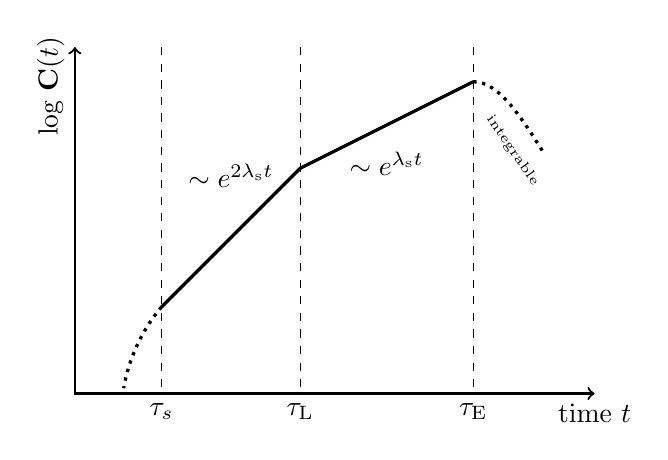
\begin{tikzpicture}[scale=2.2]
            % Draw axes
            \draw [<->,thick] (0,2) node (yaxis) [above,rotate=90,xshift=-0.5cm] {log $\mathbf{C}(t)$}
                |- (3,0) node (xaxis) [below] {time $t$};
            \draw[dashed] (0.5,2) -- (0.5,0) node[below] {$\tau_{s}$};
            \draw[dashed] (1.3,2) -- (1.3,0)  node[below] {$\tLeak$};
            \draw[dashed] (2.3,2) -- (2.3,0) node[below] {$\tEhr$};
            \draw[very thick] (0.5,0.5) -- (1.3,1.3)node [midway, above,yshift=0.5cm] {$\sim e^{2\ls t}$} -- (2.3,1.8) node [midway, below,yshift=-0.2cm] {$\sim e^{\ls t}$};
            \draw[very thick, dotted] (0.5,0.5) arc[start angle=140, end angle=170,radius=1cm] ;
            %\draw[very thick, dotted] (2.3,1.8) -- (2.9,1.8) node[midway,above] {\tiny chaotic};
            \draw[very thick, dotted] (2.3,1.8) cos (2.7,1.4);
            \draw  (2.45,1.35) node[above,rotate=-55.5] {\tiny integrable};
        \end{tikzpicture}        
        \caption{Expected behavior of an OTOC centered at a FP if~$\tLoc<\tLeak< \tEhr$: OTOCs grow polynomial for times shorter $\tLoc$, exponential with $2\ls$ for times shorter $\tLeak$, exponential with $\ls $ for times shorter $\tEhr$, but greater than $\tLeak$. Post-Ehrenfest time scales display oscillatory behaviour if the system is integrable~\cite{Fortes} and saturation if the system is chaotic \cite{Josef2018,PhysRevE.98.062218}. }
        \label{fig:SchematicOTOC_FP}
    \end{figure}
    
    It is important to note that there is a hierarchy of time scales: the leaking time is only relevant if~$\tLeak < \tEhr$, otherwise the Wigner-Weyl approximation (in leading order), see Eq.~\eqref{eq:WignerWeyl}, is already invalid. 

    The initial linear width $\Delta u$ scales with some power $\hbar_{\rm eff}^{\alpha}$ for typical states. This gives an asymptotic expression for the leaking time by $\tLeak\sim \frac{\alpha}{ \ls} \log N + O(\log(c))$. Hence, we have a direct proportional relation to the Ehrenfest time $ \tLeak \sim  \alpha\tEhr$ for $\hbarE\to 0$.
    
    We see then, that one can clearly distinguish three parametric regions: $\tLeak < \tLoc$,  $\tLoc<\tLeak < \tEhr$ and $\tEhr \leq \tLeak$ (which is equivalent to $\alpha\approx 0,<1,\approx 1$):
    \begin{enumerate}[label=\roman*)]
        \item Delocalized/uniform states: $\tLeak < \tLoc$, $\alpha\approx 0$\\
        We need to assume the FP we chose is the only unstable FP of the classical dynamics.
        Then, the OTOC is still governed by Eq.~\eqref{eq:OverviewFP} and the $e^{2\ls t}$-regime vanishes. 
        A    typical examples here are high temperature states ($T\to \infty$).
        \item Localized states:  $\tLoc<\tLeak < \tEhr$, $0< \alpha <1$\\
            In this case we have the $2\ls -\ls$ transition and asymptotically (for $N\to \infty$) we expect a sharp kink to appear at $\tLeak$.
           The prime example are the coherent states centered at a FP. They usually have a linear size of $\hbarE^{1/2}$ in all phase space directions. 
        \item Well-localized states: $\tLeak\approx \tEhr$, $\alpha \approx 1$\\
            The second $e^{\ls t}$-region is vanishing, only the one $e^{2\ls t}$-region is visible. 
            Fock states are candidates for the third class. Their linear width is $\hbarE$ in the classical occupation numbers, such that $\alpha \approx 1$ if the unstable manifold is aligned in the parallel direction.  
    \end{enumerate}
The case $\alpha>1$ is unphysical and can be excluded. The uncertainty principle requires the product of the width in all directions to be $\geq \frac{\hbarE}{2}$. Hence if $\alpha>1$, one direction must increase if $\hbarE\to 0$, i.e., this direction becomes delocalized if we approach the classical limit contradicting that the state is associated by a well-defined point in phase space. %Delocalization contradicts such a classical limit.% \rc{maybe explain why? I mean... a Fock state is delocalized and admits a classical limit in the sense of an ensemble...}.

At this point, we can explain the dynamical behavior of OTOCs reported in \cite{Hummel2019} and \cite{Scaffidi2020}. In the first paper, the authors investigated a number-projected coherent state which is simultaneously a Fock state. Its unstable manifold is parallel to the occupation direction \cite{thesisBenni}, therefore it falls into the case  iii) and they see only the $2\ls$-exponential window. Correspondingly, the authors of the second paper  use the infinite temperature state, hence their state directly falls into the first case and the only exponential window is given by $e^{\ls t}$.

In the next section, we numerically explore the validity Eq. \eqref{eq:OverviewFP} for a  Bose-Hubbard dimer, with the aim of carefully investigate the new case  ii), where the hierarchy of time scales $\tLoc<\tLeak<\tEhr$ implies, from our analysis, the presence of a $2\ls-\ls$ transition.



\section{Bose-Hubbard Dimer}
\label{sec:boseHubbard}
The Bose-Hubbard dimer describes bosonic degrees of freedom occupying on two discrete levels or sites. Prime physical setups are individual Josephson-junctions~\cite{superconductorJosephson2001} or cold atoms within a small two-sited optical lattice~\cite{Albiez2005,F_lling_2007,Witthaut2008,cheinet2008,Kierig2008,Tomkovi2017}. In all these cases, one ends with an effective description in terms of the following Hamiltonian
\begin{align}
    \label{eq:DefQuantumDimer}
\hat{H} = -2 J \big( \had{2}\ha{1}+\ha{2}\had{1} \big) + \frac{g}{2} \big( \had{1}{}^{2} \ha{1}^{2}  +\had{2}{}^{2} \ha{2}^{2}   \big),
\end{align}

where the parameter $J$ is the hopping and $g$ is the (local) interaction strength between particles given in units of energy. Our Hamiltonian differs from the usual dimer Hamiltonian, the hopping coefficient $2J$ (instead of $J$) is motivated to be consistent with a ring topology for higher number of wells. Consequently, the two-site ring has a doubled counted hopping term. We also introduce a new  dimensionless parameter~$\Theta$ with $J=\epsilon_{0}\cos \Theta$ and $g = \epsilon_{0}\frac{2}{N} \sin \Theta$. Using $\Theta$ fixes the scale of the parameters to $\epsilon_{0} = \sqrt{J^{2} + \big(\frac{gN}{2}\big)^{2}}$ in unites of an energy scale $\epsilon_{0}$. We set $\epsilon_{0}=[1]$ for a convenient unit system, that also renders the time unit $\hbar/\epsilon_{0}=1$, thus compactifying the parameter space to $\Theta \in [-\frac{\pi}{2},\frac{\pi}{2}]$.
Furthermore, this parametrization of $J$ and $g$ makes the spectrum linearly in the particle number $N$ in leading order. %\rc{Sorry man, you must introduce here physical units, as now J and g appear dimensionless}. 

\subsection{Classical mean-field limit}
We follow the standard approach \cite{negele1995quantum} to derive the classical limit for bosons and replace the operators by complex numbers 
\begin{align*}
    \ha{j}, \had{j} ~\longmapsto&~ \psi_{j},\psi^{\ast}_{j}
\end{align*}
inside the normal-ordered quantum Hamiltonian Eq.~\eqref{eq:DefQuantumDimer} to get a classical mean-field system. 
Hamilton's equations of motion $i \dot{\psi}_{j} = \frac{\partial H}{\partial \psi_{j}^{\ast}}$ define the classical dynamics.
Due to the conserved total particle number $N$, we define new set of conjugated classical variables
\begin{align*}
    \begin{matrix*}[l]
        N  =  n_1 + n_2 \,, &\phi  =  \frac{1}{2}( \varphi_1 + \varphi_2 ) \,, \\
        n  =  \frac{1}{2}( n_1 - n_2) \,, &\varphi  =  \varphi_1 - \varphi_2 - \pi \,,
    \end{matrix*}
\end{align*}
where the two mean fields $\psi_{j}=\sqrt{n_{j}}e^{i\varphi_{j}}$ are written in phase~$\varphi_{j}$ and occupations~$n_{j}$. Hence, the Hamiltonian takes the form
\begin{align}
    \begin{split}
        H(N&,\phi, n,\varphi) =
        \\
        =&\, 2\cos{\Theta} \sqrt{N^2 - 4 n^2} \cos \varphi +\sin\Theta \Big( \frac{2n^2 }{N} +  \frac{N}{2} \Big)\,.
    \end{split}
    \label{eq:classicalHamiltonian}
\end{align}
We can reduce the dynamics to an 1d-system with a single conjugated pair $(z=\frac{2n}{N},\varphi= \varphi_{1}-\varphi_{2}-\pi)$ given by the population inversion and relative phase~\cite{Campbell2020Dimer}. 
With these coordinates, we can reduce the equations of motion to two coupled real-valued ODEs
\begin{align}
    \begin{split}
        \dot{z} &= -4\cos\Theta \sqrt{1-z^{2}} \sin \varphi,
        \\
        \dot{\varphi} &=  4\cos\Theta \frac{z\cos\varphi}{\sqrt{1-z^{2}}} - 2\sin \Theta \, z,
    \end{split}
    \label{eq:EquationOfMotion}
\end{align}
%{\color{red} forgot hopping $J$ I think, multiply everything by $J= \cos(\Theta)$, to check!}
which is an 1-degree of freedom system. 
Conveniently, the mean-field system Eq. \eqref{eq:EquationOfMotion} is exactly solvable and  independent of the  particle number $N$. 


\subsection{Fixed points}

A straightforward calculation shows that there are two fixed points $(z=1$, $\varphi=\pi)$ and $(z=1$, $\varphi=0)$ which are independent from the system parameter $\Theta$. 
We call these two FPs the hom. and antihom. FP, since both have homogeneous occupations and a zero or $\pi$ phase difference between site one and two. We set the zero point for the relative phase $\varphi$ to the unstable antihom FP. 


Two bifurcations appear: at $\Theta = - \arctan 2$ for the hom. FP and at $\Theta =  \arctan 2$ for antihom. FP. 
We restrict ourselves only to the antihom. FP, since there is a symmetry between them under change of the sign of the parameter~$\Theta$.
%%%%%%%%%%%%5
 % need to check if stability analysis in the reduced form give the same diagram!!!!!
%%%%%%%%

\begin{figure}[h!]
    \centering
    \includegraphics[width=1\linewidth]{figures/L2/classical/antihomogeneousL2_antihomogeneous_stabilityExp.pdf}
    \caption{Stability exponent of the antihom. FP over the whole parameter space: change from unstable to stable at the bifurcation point $\Theta=\arctan 2$.}
    \label{fig:StablHomFP}
\end{figure}
The stability diagram of the antihom. FP in Fig. \ref{fig:StablHomFP} shows the bifurcation at $\arctan 2$, where the stability exponent becomes positive. Its maximum $\ls=0.97$ is reached at $\Theta_{\ast}\approx1.35$.

At the maximal unstable parameter $\Theta_{\ast}$, Fig.~\ref{fig:PhaseSpaceFP} shows the reduced phase space structure of the system Eq.~\eqref{eq:EquationOfMotion}. Note in particular 
the (red) separatrix defined by the unstable and stable manifold originating from the antihom. FP. The merging of stable and unstable manifolds indicates that the linearized regime is bounded, namely, any classical trajectory on the unstable manifolds converges to the stable manifold and (in infinite time) to the hyperbolic FP.
The exact size of the linearized regime (modeled by the constant $c$ in the previous Sec.~\ref{sec:OTOC_theory}) plays a neglectable role for $\hbarE\to 0$, since it is additive and $\hbarE$-independent constant in the Ehrenfest time $\tEhr$. Therefore we leave $c$ undefined in the subsequent discussion.

\begin{figure}[h!]
    \centering
    \includegraphics[width=1\linewidth]{figures/L2/classical/phase_space-dimer_piPhase_Theta1.351.pdf}
    \caption{Reduced phase space structure ($z,\varphi)$ for $\Theta_{\ast}$: contour lines of the Hamiltonian correspond to the classical trajectories, there are three stable fixed and one hyperbolic fixed point with its red dashed separatrix. Arrows on the separatrix indicate the stable and unstable manifolds.}
    \label{fig:PhaseSpaceFP}
\end{figure}


We verified that, as shown in  Fig.~\ref{fig:PhaseSpaceFP} for $\Theta_{\ast}$, we verify that this is the only unstable FP in the classical mean-field limit. This is also true for the whole range $\Theta\in (\arctan 2,\pi/2)$, where the antihom. FP is unstable.

Armed with this very specific phase-space structure, we carry an in-depth analytical study of the OTOC~$\mathbf{C}(t)$ for the dimer in the next section. 


\subsection{Microscopic approach: separatrix dynamics} 
\label{sec:peter}
\ifthenelse{1=1}
{}
{
In this section we provide a microscopic understanding of the dynamical transition by means of the exact separatrix dynamics of the mean field limit.

In this section, we work out an analytical expression for the classical OTOC
associated with a quantum state that is launched on the separatrix point of the
Bose-Hubbard dimer.
The latter is described by the quantum Hamiltonian
\begin{equation}
  \hat{H} = - J \left( \hat{a}_1^\dagger \hat{a}_2 + \hat{a}_2^\dagger \hat{a}_1
  \right) + \frac{U}{2} \sum_{l=1,2} \hat{a}_l^\dagger\hat{a}_l^\dagger
  \hat{a}_l\hat{a}_l
\end{equation}
with $\hat{a}_l^\dagger,\hat{a}_l$ the bosonic particle creation and
annihilation operator on the site $l=1,2$,
$J$ the hopping parameter, and $U$ the interaction parameter.

This quantum system has a classical counterpart which is given in terms of
the discrete nonlinear Schr\"odinger equation (setting $\hbar = 1$)
\begin{eqnarray}
  i \frac{d \psi_1}{d t} & = & - J \psi_2 + U |\psi_1|^2 \psi_1 \,, \\
  i \frac{d \psi_2}{d t} & = & - J \psi_1 + U |\psi_2|^2 \psi_2 \,,
\end{eqnarray}
with $\psi_l$ the classical field amplitude that is associated with the site
$l=1,2$.
Expressing $\psi_l = \sqrt{n_l}e^{i \varphi_l}$ in terms of the (real)
classical site occupancies $n_l$ and phases $\varphi_l$, and performing
the canonical transformation
$(n1,n2,\varphi_1,\varphi_2) \mapsto (N,n,\phi,\varphi)$
to new classical variables defined through
\begin{eqnarray}
  N & = & n_1 + n_2 \,, \\
  n & = & \frac{1}{2}( n_1 - n_2) \,, \\
  \phi & = & \frac{1}{2}( \varphi_1 + \varphi_2 ) \,, \\
  \varphi & = & \varphi_1 - \varphi_2 - \pi \,,
\end{eqnarray}
we end up with a classical Hamiltonian system described the inter-site
population exchange dynamics via the Hamiltonian
\begin{equation}
  H(n,\varphi) = U n^2 + J \sqrt{N^2 - 4 n^2} \cos \varphi \,,
  \label{eq:BH.Hc}
\end{equation}
which parametrically depends on the constant of motion $N$ corresponding
to the total population of the system.
The classical time evolution of the system is given in terms of the
Hamiltonian equations of motion
\begin{eqnarray}
  \frac{d n}{d t} & = & \frac{\partial H}{\partial \varphi}(n,\varphi) =
  - J \sqrt{N^2 - 4 n^2} \sin \varphi \,, \label{eq:BH.n} \\
  \frac{d \varphi}{d t} & = & - \frac{\partial H}{\partial n}(n,\varphi) =
  - 2 U n + \frac{4 J n \cos \varphi}{\sqrt{N^2 - 4 n^2}} \,, \label{eq:BH.ph}
\end{eqnarray}
Expressed in terms of the relative population imbalance $z = 2 n / N$,
the rescaled dimensionless time $\tau = J t$, and the dimensionless
nonlinearity parameter
\begin{equation}
  \gamma = \frac{N U}{2 J} \,,
\end{equation}
Eqs.~\eqref{eq:BH.n} and \eqref{eq:BH.ph} are rewritten as
\begin{eqnarray}
  \dot{z} \equiv \frac{d z}{d \tau} & = & - 2 \sqrt{1 - z^2} \sin\varphi \,,
  \label{eq:BH.z} \\
  \dot{\varphi} \equiv \frac{d \varphi}{d \tau} & = & - 2 \gamma z
  + \frac{2 z \cos\varphi}{\sqrt{1 - z^2}} \label{eq:BH.p} \,.
\end{eqnarray}
}
We set for the dimer the operators $\hat{A}=\hat{B}=\hat{n}_{1}$ to be the number operator $\hat{n}_{1}= \hat{a}^{\dagger}_{1} \hat{a}_{1}$ at the first site. Therefore, we get
\begin{align}
    \mathbf{C}(t) =\langle || [ \hat{n}_{1}(t), \hat{n}_{1} ] ||^2 \rangle = \langle || [ \hat{n}(t), \hat{n} ] ||^2 \rangle\, ,
    \label{eq:OTOC_defDimer}
\end{align} 
where $\hat{n} = \frac{1}{2}(\hat{n}_{1}-\hat{n}_{2})$. For this OTOC, we are interested in evaluating the classical expression which is
given by
\begin{equation}
  O(t) = \iint dn d\varphi\, W(n,\varphi)
  \left(\frac{\partial n_t}{\partial \varphi_0}\right)^2 \,, \label{eq:OTOCc}
\end{equation}
with $W(n,\varphi)$ the Wigner function associated with the initial state.
The latter is, for the sake of simplicity, modeled as a coherent quantum state
$e^{\sqrt{N_0}(\hat{a}_-^\dagger - \hat{a}_-)} \ket{0}$ with $\hat{a}_{-}=\hat{a}_{1} -\hat{a}_{2}$, keeping in mind that for large
$N_0$ this coherent state features very similar properties as a
number-projected coherent state with total particle number $N_0$ as far as the
site population exchange dynamics is concerned.
The Wigner function associated with this initial state would be given by
\begin{align}
    \begin{split}
        W(N&,\phi,n,\varphi) \simeq 
        \\
        \frac{1}{\pi^2} &\exp\left(-
        \frac{(N - N_0)^2}{2 N_0} - 2 N_0 \phi^2 - \frac{2 n^2}{N_0} -
        \frac{N_0 \varphi^2}{2} \right)
    \end{split}
\end{align}
  in the framework of a quadratic expansion valid for $N_0 \gg 1$
(using again $\hbar = 1$).
Since the Wigner function $W$ describes a tight localization of $N$ about $N_0$, we set
$N_0 = N$ henceforth and model the initial quantum state concerning the
inter-site population exchange dynamics by the Wigner function
\begin{equation}
  W(n,\varphi) = \frac{1}{\pi} \exp\left(- \frac{2 n^2}{\omega N}
  -  \frac{N \omega \varphi^2}{2} \right) \,,
\end{equation}
where the squeezing parameter $\omega$ allows for some flexibility
in the definition of the initial quantum state.

Let us first discuss the linearized dynamics in the near vicinity of
the FP~$(n,\varphi) = (0,0)$.
Linearizing Eq.~\eqref{eq:EquationOfMotion}, we obtain
the system of equations 
\begin{align}
\begin{split}
     \dot{z} & =  - 4\cos \Theta \varphi \,,  \\
  \dot{\varphi} & = - 2 (\sin \Theta -2\cos{\Theta}) z \,, 
\end{split}
\label{eq:BH.peterlinearized}
\end{align}
which is readily solved as
\begin{align}
    \begin{split}
      z_t & = z_0 \cosh \ls t - \frac{4\cos{\Theta} \varphi_0}{\ls}
      \sinh \ls t\,,  \\
      \varphi_t & = \varphi_0\cosh \ls t - \frac{\ls z_0}{4\cos{\Theta}}
      \sinh \ls t 
    \end{split}
\label{eq:BH.peterlinearizTime}
\end{align}
in terms of the stability exponent
\begin{equation}
  \ls = 4\cos{\Theta}\sqrt{\frac{\gamma}{2} - 1} \, , \label{eq:BH.la}
\end{equation}
where we defined the so called nonlinearity parameter $\gamma=\tan \Theta = \frac{gN}{LJ}$.
The latter becomes purely imaginary for $\gamma < 2$, which implies that
$(n,\varphi) = (0,0)$ turns into a stable fixed point if the nonlinearity
parameter $\gamma$ is decreased below two, as it is plotted in Fig.~\ref{fig:StablHomFP}.

Considering $\gamma > 2$ henceforth, and assuming that the point
$(z_0,\varphi_0)$ is located very closely to the origin in this phase space,
we can, as in the previous section, identify a time scale
$\tLoc \gg \ls^{-1}$ for which we still have $|z_{\tLoc}| \ll 1$ and
$|\varphi_{\tLoc}|\ll 1$, such that the above linearization Eq.~\eqref{eq:BH.peterlinearized} of the classical
equations of motion remains valid until $t = \tLoc$.
Since at the same time we have $\ls \tLoc \gg 1$ by assumption,
the solution Eq.~\eqref{eq:BH.peterlinearizTime} of the linearized
Eq.~\eqref{eq:BH.peterlinearized} for $t= \tLoc$
simplifies as
\begin{eqnarray}
  z_{\tLoc} & = & \left(\frac{z_0}{2} -  \frac{2\cos \Theta\varphi_0}{\ls}\right)
  e^{\ls \tLoc} \,, \label{eq:BH.za} \\
  \varphi_{\tLoc} & = & \left(\frac{\varphi_0}{2} - \frac{\ls z_0}{8 \cos \Theta}
  \right) e^{\ls \tLoc} \,.
\end{eqnarray}

From the time $\tLoc$ on, we can safely assume that the trajectory
under consideration very closely follows the separatrix structure emanating
from the unstable antihom. fixed point $(z,\varphi) =(0,0)$. 
This separatrix structure is obtained through the identification of the
energy
\begin{equation}
  H(n,\varphi) = 2\cos \Theta N + \sin{\Theta} \frac{N}{2}
\end{equation}
of the classical Hamiltonian Eq. \eqref{eq:classicalHamiltonian}, from which follows the identity
\begin{equation*}
  \cos\varphi = \frac{1 - \frac{\gamma}{4} z^2 }{\sqrt{1 - z^2}} \,.
\end{equation*}
Inserting this expression into Eq.~\eqref{eq:EquationOfMotion} yields the differential
equation
\begin{equation*}
  \dot{z} = z \sqrt{\ls^2 - \sin^2\Theta  z^2}
\end{equation*}
describing the motion along the upper or lower separatrix branch.
This equation is straightforwardly integrated yielding
\begin{align*}
  t - \tLoc =& \int_{z_{\tLoc}}^{z_t}
  \frac{\d z}{z \sqrt{\ls^2 - \sin^2\Theta z^2}}
  \\
   =& - \frac{1}{\ls}\left[ \mathrm{arcosh}
    \left(\frac{\ls}{\sin \Theta |z_{t}|} \right) - \mathrm{arcosh}
    \left(\frac{\ls}{\sin \Theta |z_{\tLoc}|} \right) \right] \,,
\end{align*}
from which we obtain
\begin{equation}
  z_t= \frac{\mathrm{sgn}(z_{\tLoc}) \ls / \sin\Theta}
  {\cosh\left[\mathrm{arcosh} \left(\frac{\ls}{\sin\Theta |z_{\tLoc}|}
      \right) - \ls (t - \tLoc) \right]} \,.
      \label{eq:zt}
\end{equation}
Using $|z_{\tLoc}| \ll 1$ and hence also $\sin\Theta |z_{\tLoc}|/\ls \ll 1$
for finite values of $\sin\Theta$ and $\ls$, we define
\begin{align}
  \begin{split}
    x_t & = \mathrm{sgn}(z_{\tLoc})\exp\left[-\mathrm{arcosh}
    \left(\frac{\ls}{\gamma |z_{\tLoc}|}\right) + \ls (t - \tLoc)
    \right]  
    \\
  & \simeq  \frac{\sin \Theta}{2 \ls} \left(\frac{z_0}{2} -
  2\cos \Theta\frac{\varphi_0}{\ls}\right)e^{\ls t} 
  \\
  &\simeq
  \frac{\sin \Theta}{\ls} \left(\frac{n_0}{N} - 2\cos \Theta
  \frac{\varphi_0}{\ls}\right)\sinh(\ls t) \,, 
  \end{split}
  \label{eq:xt}
\end{align}
where we make use of the asymptotic expression
\begin{equation}
  \mathrm{arcosh}(u) = \ln\left(u + \sqrt{u^2 - 1}\right) \simeq \ln(2u)
   + O(u^{-2})
   \label{eq:arcosh}
\end{equation}
for large $u$, in combination with Eq.~\eqref{eq:BH.za}.
With $(\cosh u)^{-1} = 2 e^u / ( 1 + e^{2u})$ together with Eqs.~\eqref{eq:arcosh} and \eqref{eq:xt}, Eq.~\eqref{eq:zt} yields
\begin{equation}
  z_\tau = \frac{2 \ls}{\sin \Theta} \frac{x_t}{1 + x_t^2}
\end{equation}
and thus
\begin{equation}
  n_t = \frac{N \ls}{\sin \Theta} \frac{x_{t}}{1 + x_{t}^2}
  \label{eq:BH.nt} \,.
\end{equation}
Replacing $e^{\ls t}$ with $2 \sinh(\ls t)$ in Eq.~\eqref{eq:xt}
is clearly valid for large $\ls t\gg 1$ and has the additional advantage
that the short-time regime in the time evolution of $n_t$ will thereby be
correctly captured as well within Eq.~\eqref{eq:BH.nt}.

The classical limit of the quantum OTOC, Eq.~\eqref{eq:OTOCc},
is then evaluated as
\begin{align}
    \begin{split}
    O(t) = \frac{2\cos^2\Theta N^2}{ \sqrt{\pi} a \ls^2}& \sinh(\ls t)
    \\
  \int \frac{(1 - x^2)^2}{(1 + x^2)^4}&
  \exp\left[-\left(\frac{ x}{2a \sinh(\ls t)}\right)^2\right] \d x 
    \end{split}
    \label{eq:exact.clOTOC}
\end{align}
where the dimensionless scale is defined as
\begin{equation}
  a = \frac{\sin{\Theta}/\ls}{\sqrt{8 \omega N}}
  \sqrt{\omega^2 + \frac{16 \cos^2 \Theta }{\ls^2}} \,.
  \label{eq:aParameter}
\end{equation}
% Using Eq.~\eqref{eq:BH.la}, this expression simplifies in the special
% case $\omega = 1$ yielding
% \begin{equation}
%   a = \frac{1}{\gamma - 1}\sqrt{\frac{\gamma^3}{32 N}}
%   = \frac{N \sqrt{U^3/J}}{8(N U - 2 J)} \,.
% \end{equation}
The short-time behavior of the OTOC, for $t \ll \tLeak = - \ls^{-1} \ln a$,
is yielded as
\begin{equation}
  O(t) \simeq 4\cos^{2} \Theta \frac{N^2}{\ls^2} \sinh^2(\ls t) \,,
  \label{eq:shortClassical}
\end{equation}
while for $t \gg \tLeak$ we obtain
\begin{equation}
  O(t) \simeq \cos^{2} \Theta \frac{\sqrt{\pi} N^2}{4 a \ls^2} e^{\ls t} \,.
  \label{eq:longClassical}
\end{equation}
These two limits correspond to the heuristic derived $2\ls-\ls$ transition Eq.~\eqref{eq:OverviewFP} in the previous Sec.~\ref{sec:OTOC_theory}. Note the here defined $\tLeak$ agrees with the case ii) in Sec.~\ref{sec:OTOC_theory}.
The dimensionless constant $\ln a$ encodes the linear width of the wave-packet along the unstable direction. 

With this extensive classical calculation at hand, we analyze the OTOC centered around this local hyperbolic antihom. FP using $\Theta_{\ast}$ at the maximal value of the stability exponent $\ls = 0.97$. 

\subsection{Numerical results for the Out-of-Time-Order Correlator}


We proceed now with the numerical study and calculate the OTOC via Eq.~\eqref{eq:OTOC_defDimer} by means of extensive numerically exact simulations for the operators $\hat{A}=\hat{B}=\hat{n}_{1}$. We will consider the state 
\begin{align*}
    |{\vec{\xi}}\,\rangle = \frac{1}{\mathcal{N}} \big( \Vec{\xi}\cdot \hat{\vec{a}}^{\dagger} \big)^{N} \ket{0},
\end{align*}
which is a number-projected coherent state centered at the antihom. FP $\vec{\xi} = (\sqrt{N/2},-\sqrt{N/2})$, with $\mathcal{N} = \sqrt{N^N N!}$ a normalization constant.

For large total particle number $N$, the projected coherent state inherits properties from the coherent state, in particular the linear width of $\hbar_{{\rm eff}}^{1/2}$ in each phase space direction \cite{gardiner2004quantum}, including the unstable direction in Fig.~\ref{fig:PhaseSpaceFP}. Furthermore it sets the squeezing parameter $\omega=1$ in the classical analysis in Eq.~\eqref{eq:aParameter}. 
Following the discussion in Sec.~\ref{sec:OTOC_theory}, case ii), the leaking time $\tLeak$ is therefore half the Ehrenfest time $\tEhr$.
\begin{figure}[h!]
    \centering
    \includegraphics[width=\linewidth]{figures/L2/OTOC-plots/OTOC_antihomogeneous_N1000_L2_Theta1.351.pdf}\\
    \includegraphics[width=\linewidth]{figures/L2/OTOC-plots/OTOC_antihomogeneous_N10000_L2_Theta1.351.pdf}\\
    \includegraphics[width=\linewidth]{figures/L2/OTOC-plots/OTOC_antihomogeneous_N50000_L2_Theta1.351.pdf}
    %\includegraphics[width=0.75\linewidth,page=1]{figures/L2/OTOC-plots/comb_Theta=-1.35_N=1000_L=2.pdf}\\
    %\includegraphics[width=0.75\linewidth,page=1]{figures/L2/OTOC-plots/comb_Theta=-1.35_N=10000_L=2.pdf}\\
    %\includegraphics[width=0.75\linewidth,page=1]{figures/L2/OTOC-plots/comb_Theta=-1.35_N=50000_L=2.pdf}
    \caption{Top to bottom: OTOC $\mathbf{C}(t)$ for $N=10^3, ~10^4, ~5\cdot 10^4$ and $\Theta=1.35$; shaping kink from the $2\ls-\ls$ transition at $\tLeak=\tEhr/2$;  the classical expressions Eq.~\eqref{eq:shortClassical} and Eq.~\eqref{eq:longClassical} fit tightly the OTOC in each region showing $e^{2\ls t}$ and $e^{\ls t}$ exponential growth rates.}
    \label{fig:OTOC_FP_numeric}
\end{figure}
 We display our numerical OTOCs for increasing particle $N=10^3, ~10^4, ~5\cdot 10^4$ in Fig.~\ref{fig:OTOC_FP_numeric}, where we observe the predicted $2\ls-\ls$ transition, precisely following the heuristic arguments of Sec.~\ref{sec:OTOC_theory} and the exact analysis of Sec.~\ref{sec:peter}. In particular, the analytical result for the classical OTOC Eq.~\eqref{eq:exact.clOTOC} follows perfectly the quantum OTOC $\mathbf{C}(t)$, i.e., it captures both regimes and the transition.
 The kink at the transition gets sharper for $N\to \infty$.  Here, the insets showing the time-derivative of $\log (\mathbf{C}(t))$ confirm a more and more pronounced $2\ls$ and $\ls$ regions of exponential growth.


\begin{figure*}[!ht]
    \centering
    %\includegraphics[width=0.35\linewidth,page=21,trim ={ 1.2cm 1.9cm 7.5cm 1.75cm},clip]{figures/L2/Husimi-phase-space/Husimi_log_hom_Theta=-1.35_N=1000_L=2-1.pdf}%
    %\includegraphics[width=0.35\linewidth,page=26,trim ={ 1.2cm 1.9cm 7.5cm 1.75cm},clip]{figures/L2/Husimi-phase-space/Husimi_log_hom_Theta=-1.35_N=1000_L=2-1.pdf}
    %\\
    %\includegraphics[width=0.35\linewidth,page=31,trim ={ 1.2cm 1.9cm 7.5cm 1.75cm},clip]{figures/L2/Husimi-phase-space/Husimi_log_hom_Theta=-1.35_N=1000_L=2-1.pdf}%
    %\includegraphics[width=0.35\linewidth,page=36,trim ={ 1.2cm 1.9cm 7.5cm 1.75cm},clip]{figures/L2/Husimi-phase-space/Husimi_log_hom_Theta=-1.35_N=1000_L=2-1.pdf}
    \includegraphics[width=0.5\linewidth,page=21,clip]{figures/L2/Husimi-phase-space/antihom_comb_Theta=1.35_N=1000_L=2.pdf}%
    \includegraphics[width=0.5\linewidth,page=26,clip]{figures/L2/Husimi-phase-space/antihom_comb_Theta=1.35_N=1000_L=2.pdf}%
    \\
    \includegraphics[width=0.5\linewidth,page=31,clip]{figures/L2/Husimi-phase-space/antihom_comb_Theta=1.35_N=1000_L=2.pdf}%
    \includegraphics[width=0.5\linewidth,page=36,clip]{figures/L2/Husimi-phase-space/antihom_comb_Theta=1.35_N=1000_L=2.pdf}%
    
    %\includegraphics[width=0.35\linewidth,page=31,trim ={ 1.2cm 1.9cm 7.5cm 1.75cm},clip]{figures/L2/Husimi-phase-space/Husimi_log_hom_Theta=-1.35_N=1000_L=2-1.pdf}%
    %\includegraphics[width=0.35\linewidth,page=36,trim ={ 1.2cm 1.9cm 7.5cm 1.75cm},clip]{figures/L2/Husimi-phase-space/Husimi_log_hom_Theta=-1.35_N=1000_L=2-1.pdf}
    
    \caption{Time-evolution of the Husimi-distribution for the state $|\vec{\xi}\, \rangle$ centered at the hyperbolic antihom. FP with $N=10^3$ particles, we observe scrambling along the unstable manifold on the separatrix until $t\approx \tLeak$.}
    \label{fig:husimiFP}
\end{figure*}
In order to justify the leaking from the linearized region around the FP, we visualize the time dynamical evolution of the Husimi distribution for $N=10^{3}$ in Fig.~\ref{fig:husimiFP}. 
With time, the linear width of the wave-packet increases and evolves to the upper right and lower left corner of the phase space. 
We recognize that at time $\tLeak = \tEhr/2$ the wave-packet folds back from the unstable to the stable manifold. 
This back-folding corresponds to the dynamical transition of leaking from the linearized regime.

The excellent agreement between our physical picture based on the leaking mechanism and the numerical simulations opens the possibility of manipulating the leaking time $\tLeak$, and therefore the different scrambling regimes, via squeezing the initial state $|{\vec{\xi}}\,\rangle$, as we discuss next.


\subsection{Squeezing -- engineering the leaking time $\tLeak$}

%\rc{Jesus Christ, what the hell means "A further manifest of our theory"?}
An important consequence of the leaking mechanism is that the linear width of the initial state along the unstable manifolds is the key ingredient for the exact position of the $2\ls-\ls$ transition. 

In order to check this dependence, we proceed to squeeze the coherent state on the antihom. FP and subsequently calculate the OTOC. Interestingly, squeezed states in optical lattices can be archived experimentally \cite{squeezingBEC2008} to an excellent degree. In our theoretical setup, squeezing protocol can be effectively (and unitarily) realized by the reversing the time evolution itself. This means, we replace $\ket{\xi }$ by 
\begin{align*}
    \ket{\xi (t_{0})} = \hat{U}(t_{0})\ket{\xi}
\end{align*}
with $t_{0} = -\tEhr/2$, where $\hat{U}(t_{0})$ is the time-evolution operator, and then  calculate the OTOC Eq.~\eqref{eq:OTOC_def} for the initial state $\hat{\rho}(t_{0}) = \ket{\xi (t_{0}) }\bra{\xi (t_{0})} $. The corresponding scrambling dynamics is shown in then the left panel of Fig. \ref{fig:OTOC_FP_numeric_squeezed} for $N=10^3$, while the right panel depicts the initial Husimi distribution of the squeezed state.
\begin{figure*}[th!]
    \centering
    \includegraphics[width=0.49\linewidth,page=11]{figures/L2/OTOC-plots/timeShift_antihom_Theta=1.35_N=1000_L=2.pdf}%
    %\includegraphics[width=0.54\linewidth,page=16]{figures/L2/OTOC-plots/timeShift_t0_Theta=-1.35_N=1000_L=2.pdf}%
    %\includegraphics[width=0.46\linewidth,page=7]{figures/L2/Husimi-phase-space/Husimi_log_hom_Theta=-1.35_N=1000_L=2-1.pdf}
    \includegraphics[width=0.51\linewidth,page=11,clip]{figures/L2/Husimi-phase-space/antihom_comb_Theta=1.35_N=1000_L=2.pdf}%
    \caption{Left panel: OTOC for a squeezed coherent state for the system parameter $\Theta=1.35$ and particle number $N=10^{3}$; the transition to $\ls$ vanishes. Right panel: Husimi distribution of the squeezed coherent state. The state is distributed along the stable and localized $\sim \hbarE$ along the unstable manifold.}
    \label{fig:OTOC_FP_numeric_squeezed}
\end{figure*}
This backward-time evaluated coherent state has a reduced linear width along the unstable manifold by taking $t_{0}$ to $-\tEhr/2$ (for the non-squeezed coherent state), i.e., we transform $\Delta u \sim \hbar_{{\rm eff}}^{1/2}$ to $\Delta u \sim \hbarE$. Thus, the new leaking time $\tLeak^{\ast}$ is at the Ehrenfest time and no $2\ls-\ls$~transition is expected to exist, as fully confirmed by the numerical simulations.

\subsection{OTOC -- parameter scan }
So far, we handpicked one of the most unstable configuration for the antihom. FP and did not perform a fitting with an exponential function beyond the visual agreement in Figs.~\ref{fig:OTOC_FP_numeric} and ~\ref{fig:OTOC_FP_numeric_squeezed}. 
We now show the results of a proper fitting procedure in Fig. \ref{fig:parameterScan}  for the number projected state $|{\vec{\xi}}\,\rangle$. Here, we show the fitted quantum Lyapunov exponents $\lq$ of the OTOC in both regions $[\tLoc,\tLeak]$ and $[\tLeak,\tEhr]$ along the whole parameter range of $\Theta$ and for several values of the total particle number $N$.  
We see an increasing agreement with the $2\ls$- and $\ls$-regions: the fitted exponents show the same $\Theta$-dependency as the stability exponent $\ls$. Further, their magnitudes approach the classical value with $\hbarE\to 0$. The discrepancy originates from the fitting procedure, as it ignores the transition between the two exponential regimes. 
\begin{figure*}[]
    \centering
    \includegraphics[width=0.5\linewidth]{figures/L2/parameter-Fits/antihomogeneousL2_antihomogeneous_fitShort.pdf}%
    \includegraphics[width=0.5\linewidth]{figures/L2/parameter-Fits/antihomogeneousL2_antihomogeneous_fitLong.pdf}
    %\includegraphics[width=0.8\linewidth]{figures/L2/parameter-Fits/homogeneousL2_N[10, 100, 1000, 10000, 40000]_firstWindow.pdf}\\
    %\includegraphics[width=0.8\linewidth]{figures/L2/parameter-Fits/homogeneousL2_N[10, 100, 1000, 10000, 40000]_secondWindow.pdf}
    \caption{Fitted exponents for the $2\ls$ (upper panel) and the~$\ls$ (lower panel) region; for $N\to \infty$, we see an increasing agreement with the classical predictions from Eq.~\eqref{eq:OverviewFP}.}
    \label{fig:parameterScan}
\end{figure*}
We conclude that the~$2\ls-\ls$ transition is independent of the specific value of~$\Theta$, i.e., it is a robust signal of a dynamical transition.
%\FloatBarrier

\section{Conclusions}
We consider the phase-extraction problem, and we showed that, given a unitary $U = e^{i\pi H}$ and its inverse $U^{\dag}$, we could implement a block-encoding of $\phi(H)$ for some smooth function $\phi(x)$. The word `smooth' here means existence and continuity of the derivatives: the higher the number of continuous derivatives that a function has, the faster its Fourier sum (and thus the Laurent polynomial on the eigenphases) uniformly converges to that function. We are confident this can have many more applications beyond what is shown in this work. It is also worth remarking that Jackson showed that the convergence rate of a Fourier series is almost-optimal, in the sense that no trigonometric (or, equivalently, complex exponential) series can approximate the desired function faster, up to that $\log d$ factor~\cite[p.\ 21]{jacksonTheoryApproximation1930a}. Also remember that `smoothing' a function, i.e., replacing its derivative with a continuous function, does not give faster convergence for free in general, as its derivative will become steep in the points where we smooth out discontinuities, and this translates to a high Lipschitz constant: a~clear example is given by Eq.~\ref{eq:lipschitz-constant-recurrence-solution}, but in that case, fortunately, nothing depends on the size of the input $N$, and thus does not influence the asymptotic query complexity of Algorithm~\ref{alg:prop-sampling-qsp}, although the constant factor can become large even for $p = 20$. From a theoretical point of view, this work shows that, for any $\eta > 0$, there is an algorithm with query complexity 
$$\Tilde{\bigO}\left(\frac{1}{\bar{c}^{\frac{1}{2} + \eta}} \frac{1}{\epsilon^\eta} \right)$$
solving the proportional-sampling problem. This statement seems to suggest there exists an algorithm which directly solves the problem with $\eta = 0$, and an open question would be to find such algorithm.


It is also interesting to remark that Theorems~\ref{thm:haah-construction},~\ref{thm:haah-completion} indeed allow the construction for any $\phi$, even complex-valued, provided that its absolute value is reciprocal.

One could think that, in Section~\ref{sec:prop-sampling}, instead of using the linear function in the phase-extraction subroutine, we could approximate the square root and then apply the transformation directly on $e^{i \pi c(x)}$. However, in the case of proportional sampling this would be inconvenient, as the derivative of the square root function has a discontinuity with an infinite jump around 0, and we could not choose a constant $\delta$ if we had values of the oracle that are too close to $0$.
\chapter*{Acknowledgement}
\addcontentsline{toc}{chapter}{Acknowledgement}
The authors thank Andrzej Kupsc, Sergey Barsuk, Olivier Callot and Wolfgang K{\"u}hn for their contribution on the CDR draft.
%The authors thank the international review committee XXX for their great effort in reading the CDR draft and providing valuable suggestions. 
The STCF working group thanks all 
the colleagues in the world-wide community for many profitable discussions
and expresses gratitude to the Hefei Comprehensive National Science Center for their strong support.  This work is supported by: international 
partnership program of the Chinese Academy of Sciences Grant No. 211134KYSB20200057.
%\section{Appendix for Proofs}

\paragraph{Proof of Theorem \ref{thm:main}.}

\begin{proof}
\label{proof:main}
Our proof has two steps. In Step 1, we will show that SimCLR is equivalent to minimizing the cross entropy loss defined in Eqn.~(\ref{eqn:cross-entropy}). 
In Step 2, we will show  that minimizing the cross-entropy loss 
is equivalent to spectral clustering on $\bfpi$. 
Combining the two steps together, we have proved our theorem. 

\textbf{Step 1: } SimCLR is equivalent to minimizing the cross entropy loss.

The cross-entropy loss takes expectation over 
$\bfW_\bfX\sim \mathbb{P}(\cdot ; \bfpi)$, 
which means $\bfW_\bfX$ has exactly one non-zero entry in each row $i$. By Lemma~\ref{lem:multinomial}, we know every row $i$ of $\bfW_\bfX$ is independent of other rows. Moreover, 
$\bfW_{\bfX,i}\sim \mathcal{M}(1, \bfpi_i/\sum_j \bfpi_{i,j})=\mathcal{M}(1, \bfpi_i)$, because $\bfpi_i$ itself is a probability distribution.
Similarly, we know $\bfW_\bfZ$ also has the row-independent property by sampling over $\mathbb{P}(\cdot;\bfK_\bfZ)$.
Therefore, by Lemma~\ref{lem:cross_split}, we know Eqn.~(\ref{eqn:cross-entropy}) is equivalent to:
\[
 -\sum_{i=1}^n \mathbb{E}_{\bfW_{\bfX,i}}[\log \mathbb{P}(\bfW_{\bfZ,i}=\bfW_{\bfX,i};\bfK_\bfZ)],
\]

This expression takes expectation over $\bfW_{\bfX,i}$ for the given row $i$. Notice that 
$\bfW_{\bfX,i}$ has exactly one non-zero entry, which equals $1$ (same for $\bfW_{\bfZ,i}$). 
As a result
we expand the above expression to be:
\begin{equation}
 -\sum_{i=1}^n \sum_{j\neq i} \Pr(\bfW_{\bfX,i,j}=1)\log \Pr(\bfW_{\bfZ,i,j}=1).
\label{eqn:detailed-expansion}    
\end{equation}


By Lemma~\ref{lem:multinomial}, $\Pr(\bfW_{\bfZ,i,j}=1)=\bfK_{\bfZ,i,j}/\|\bfK_{\bfZ,i}\|_1$ for $j\neq i$. Recall that $\bfK_\bfZ=(k(\bfZ_i-\bfZ_j))_{(i,j)\in[n]^2}$, which means 
$\bfK_{\bfZ,i,j}/\|\bfK_{\bfZ,i}\|_1=\frac{\exp(-\|\bfZ_i-\bfZ_j\|^2/{2\tau})}{\sum_{k\neq i}
\exp(-\|\bfZ_i-\bfZ_k\|^2/{2\tau})
}$ for $j\neq i$, when $k$ is the Gaussian kernel with variance $\tau$. 

Notice that $\bfZ_i=f(\bfX_i)$, so we know
\begin{equation}
-\log \Pr(\bfW_{\bfZ,i,j}=1)=
-\log \frac{\exp(-\|f(\bfX_i)-f(\bfX_j)\|^2/{2\tau})}{\sum_{k\neq i}
\exp(-\|f(\bfX_i)-f(\bfX_k)\|^2/{2\tau}),
}
\label{eqn:infonce-equivalence}    
\end{equation}


The right hand side is exactly the InfoNCE loss defined in Eqn.~(\ref{eqn:infonce}).
Inserting Eqn.~(\ref{eqn:infonce-equivalence}) into Eqn.~(\ref{eqn:detailed-expansion}), we get the SimCLR algorithm, which first samples augmentation pairs $(i,j)$ with $\Pr(\bfW_{\bfX,i,j}=1)$ for each row $i$, and then optimize the InfoNCE loss. 

\textbf{Step 2: } minimizing the cross entropy loss 
is equivalent to spectral clustering on $\bfpi$.


By Lemma~\ref{lem:convert_to_spectral}, we may further convert the loss to 
\begin{equation}
\label{eqn:main-theorem-repul-attr}
\min_{\bfZ}
-\sum_{(i,j)\in [n]^2} \mathbf{P}_{i,j}
\log k (\bfZ_i-\bfZ_j)+\log \mathbf{R}(\bfZ).
\end{equation}
Since $k$ is the Gaussian kernel, this reduces to \[
\min_\bfZ \mathrm{tr}(\bfZ^\top \mathbf{L}(\bfpi) \bfZ)
+\log \mathbf{R}(\bfZ),
\]

where we use the fact that $\mathbb{E}_{\bfW_\bfX\sim \mathbb{P}(\cdot; \bfpi)}[\mathbf{L}(\bfW_\bfX)]
=\mathbf{L}(\bfpi)
$, because the Laplacian operator is linear and $
\mathbb{E}_{\bfW_\bfX\sim \mathbb{P}(\cdot; \bfpi)}(\bfW_\bfX)=\bfpi
$.
\end{proof}

\paragraph{Proof of Theorem \ref{thm:clip}.}
\begin{proof}
Since $\bfW_\bfX\sim \mathbb{P}(\cdot;\bfpi_{\mathbf{A}, \mathbf{B}})$, we know 
$\bfW_\bfX$ has exactly one non-zero entry in each row, denoting the pair that got sampled. 
A notable difference compared to the previous proof is we now have $n_\mathcal{A}+n_\mathcal{B}$ objects in our graph. CLIP deals with this by taking a mini-batch of size $2N$, 
such that $n_\mathcal{A}=n_\mathcal{B}=N$, and adding the $2N$ InfoNCE losses together. We label the objects in $\mathcal{A}$ as $[n_\mathcal{A}]$, and the objects in $\mathcal{B}$ as $\{n_\mathcal{A}+1, \cdots, n_\mathcal{A}+n_\mathcal{B}\}$. 

Notice that $\bfpi_{\mathbf{A}, \mathbf{B}}$ is a bipartite graph, so the edges of objects in $\mathcal{A}$ will only connect to object in $\mathcal{B}$ and vice versa. We can define the similarity matrix in $\cZ$ as $\bfK_\bfZ$, 
where $\bfK_\bfZ(i, j+n_\mathcal{A})=\bfK_\bfZ(j+n_\mathcal{A},i)= k(\bfZ_i-\bfZ_j)$ for $i\in [n_\mathcal{A}], j\in [n_\mathcal{B}]$, and otherwise we set $\bfK_\bfZ(i,j)=0$. 
The rest is same as the previous proof. 
\end{proof}

\paragraph{Proof of Theorem \ref{thm:exponential}.}

\begin{proof}
\label{proof:exponential}
Since the objective function consists of a linear term combined with an entropy regularization, which is a strongly concave function, the maximization problem is a convex optimization problem. Owing to the implicit constraints provided by the entropy function, the problem is equivalent to having only the equality constraint. We then introduce the Lagrangian multiplier $\lambda$ and obtain the following relaxed problem:

$$
\widetilde{E}(\boldsymbol{\alpha})=\psi_{1}-\sum_{i=1}^n \alpha_{i} \psi_{i}+\tau \sum_{i=1}^n \alpha_{i}\log \alpha_{i}+\lambda\left(\boldsymbol{\alpha}^{\top} \mathbf{1}_n-1\right).
$$

As the relaxed problem is unconstrained, taking the derivative with respect to $\alpha_{i}$ yields

$$
\frac{\partial \widetilde{E}(\boldsymbol{\alpha})}{\partial \alpha_{i}}=-\psi_{i}+\tau\left(\log \alpha_{i}+\alpha_{i} \frac{1}{\alpha_{i}}\right)+\lambda=0.
$$

Solving the above equation implies that $\alpha_{i}$ takes the form
$
\alpha_{i}=\exp \left(\frac{1}{\tau} \psi_{i}\right) \exp \left(\frac{-\lambda}{\tau}-1\right).
$ Since $\alpha_{i}$ lies on the probability simplex, the optimal $\alpha_{i}$ is explicitly given by
$
\alpha^{*}_{i}=\frac{\exp \left(\frac{1}{\tau} \psi_{i}\right)}{\sum_{i^{\prime}=1}^n \exp \left(\frac{1}{\tau} \psi_{i^{\prime}}\right)} .
$ Substituting the optimal point into the objective function, we obtain
$$
\begin{aligned}
E\left(\boldsymbol{\alpha}^*\right)  &=\psi_1-\sum_{i=1}^n \frac{\exp \left(\frac{1}{\tau} \psi_{i}\right)}{\sum_{i^{\prime}=1}^n \exp \left(\frac{1}{\tau} \psi_{i^{\prime}}\right)} \psi_{i}+\tau \sum_{i=1}^n \frac{\exp \left(\frac{1}{\tau} \psi_{i}\right)}{\sum_{i^{\prime}=1}^n \exp \left(\frac{1}{\tau} \psi_{i^{\prime}}\right)}\log \frac{\exp \left(\frac{1}{\tau} \psi_{i}\right)}{\sum_{i^{\prime}=1}^n \exp \left(\frac{1}{\tau} \psi_{i^{\prime}}\right)} \\
& =\psi_1 - \tau \log \left(\sum_{i=1}^n \exp \left(\frac{1}{\tau} \psi_{i}\right)\right).
\end{aligned}
$$
Thus, the Lagrangian dual function is given by
\begin{equation*}
-E\left(\boldsymbol{\alpha}^*\right)= -\tau \log \frac{\exp \left(\frac{1}{\tau} \psi_{1}\right)}{\sum_{i=1}^n \exp \left(\frac{1}{\tau} \psi_{i}\right)}.\qedhere
\end{equation*}
\end{proof}



\section{More on Experiments} \label{section: experiment_details}

\paragraph{CIFAR-10 and CIFAR-100} CIFAR-10 ~\citep{krizhevsky2009learning} and CIFAR-100 ~\citep{krizhevsky2009learning} are well-known classic image classification datasets. Both CIFAR-10 and CIFAR-100 contain a total of 60k $32 \times 32$ labeled images of different classes, with 50k for training and 10k for testing. CIFAR-10 is similar to CIFAR-100, except there are 10 different classes in CIFAR-10 and 100 classes in CIFAR-100.

\paragraph{TinyImageNet} TinyImageNet ~\citep{le2015tiny} is a subset of ImageNet ~\citep{deng2009imagenet}. There are 200 different object classes in TinyImageNet, with 500 training images, 50 validation images, and 50 test images for each class. All the images in TinyImageNet are colored and labeled with a size of $64 \times 64$.

\textbf{Pseudo-code.} Algorithm \ref{alg:Training Procedure} presents the pseudo-code for our empirical training procedure.

\begin{algorithm}[!htbp]
\caption{Training Procedure}
\label{alg:Training Procedure}
\begin{algorithmic}[1]
\REQUIRE trainable encoder network $f$, batch size $N$, augmentation strategy \textit{aug}, loss function $L$ with hyperparameters \textit{args}
\FOR {sampled minibatch ${x_i}_{i=1}^N$}
\FORALL{$i \in { 1, ..., N }$}
\STATE draw two augmentations $t_i = \textit{aug}\left(x_i\right) $, $t_i' = \textit{aug}\left(x_i\right) $
\STATE $z_i = f\left(t_i\right)$, $z_i' = f\left(t_i'\right)$
\ENDFOR
\STATE compute loss $\mathcal{L} = L(N, z, z', \textit{args})$
\STATE update encoder network $f$ to minimize $\mathcal{L}$
\ENDFOR
\STATE \textbf{Return} encoder network $f$
\end{algorithmic}
\end{algorithm}

We also provide the pseudo-code for our core loss function used in the training procedure in Algorithm \ref{alg:Core loss}. The pseudo-code is almost identical to SimCLR's loss function, with the exception of an extra parameter $\gamma$.

\begin{algorithm}[!htbp]
\caption{Core loss function $\mathcal{C}$}
\label{alg:Core loss}
\begin{algorithmic}[1]
\REQUIRE batch size $N$, two encoded minibatches $z_1, z_2$, $\gamma$, temperature $\tau$
\STATE $z = \textit{concat}\left(z_1, z_2\right)$
\FOR {$i \in {1, ..., 2N }, j \in {1, ..., 2N}$ }
\STATE $s_{i,j} = \Vert z_i - z_j \Vert_2^{\gamma}$
\ENDFOR
\STATE \textbf{define} $l(i, j)$ \textbf{as} $l(i, j) = - \log \frac{exp\left(s_{i,j}/\tau \right)}{\sum_{k=1}^{2N} \mathbf{1}{[k \ne i]} exp\left(s{i, j} / \tau \right)} $
\STATE \textbf{Return} $\frac{1}{2N} \sum_{k=1}^N\left[l(i, i+N) + l(i+N, i)\right]$
\end{algorithmic}
\end{algorithm}

Utilizing the core loss function $\mathcal{C}$, we can define all kernel loss functions used in our experiments in Table \ref{table: loss definition}. For all $z_i \in z$ with even dimensions $n$, we define $z_{L_i} = z_i\left[0:n/2\right]$ and $z_{R_i} = z_i\left[n/2:n\right]$.

\begin{table}[ht]
\centering
\begin{tabular}{{@{}l|l@{}}}
Kernel  &  Loss function \\ \midrule
Laplacian & $\mathcal{C}\left(N, z, z', \gamma=1, \tau\right)$\\ \midrule
Sum       & $\lambda * \mathcal{C}\left(N, z, z', \gamma=1, \tau_1\right) + (1-\lambda) * \mathcal{C}\left(N, z, z', \gamma=2, \tau_2\right)$  \\ \midrule
Concatenation Sum&$\lambda * \mathcal{C}\left(N, z_L, z'_L, \gamma=1, \tau_1\right) + (1-\lambda) * \mathcal{C}\left(N, z_R, z'_R, \gamma=2, \tau_2\right)$\\ \midrule
$\gamma = 0.5$ & $\mathcal{C}\left(N, z, z', \gamma=0.5, \tau\right)$          \\ 

\end{tabular}

\caption{Definition of kernel loss functions in our experiments}
\label {table: loss definition}
\end{table}

\textbf{Baselines.} We reproduce the SimCLR algorithm using PyTorch Lightning~\citep{PytorchLightning}.

\textbf{Encoder details.}
The encoder $f$ consists of a backbone network and a projection network. We employ ResNet50~\citep{ResNet} as the backbone and a 2-layer MLP (connected by a batch normalization~\citep{ioffe2015batch} layer and a ReLU \cite{nair2010rectified} layer) with hidden dimensions 2048 and output dimensions 128 (or 256 in the concatenation kernel case).

\textbf{Encoder hyperparameter tuning.}
For each encoder training case, we randomly sample 500 hyperparameter groups (sample details are shown in Table \ref{table: Hyperparameter sample}) and train these samples simultaneously using Ray Tune ~\citep{RayTune}, with the ASHA scheduler~\citep{li2018massively}. Ultimately, the hyperparameter group that maximizes the online validation accuracy (integrated in PyTorch Lightning) within 5000 validation steps is chosen for the given encoder training case.

\begin{table}[ht]
\centering

\begin{tabular}{@{}l|l|l@{}}
\midrule
Hyperparameter  & Sample Range & Sample Strategy \\ \midrule
start learning rate & $\left[10^{-2}, 10\right]$ & log uniform \\ \midrule
$\lambda$       & $\left[0, 1\right]$ & uniform \\ \midrule
$\tau$, $\tau_1$, $\tau_2$ & $\left[0, 1\right]$ & log uniform \\ \midrule
\end{tabular}

\caption{Hyperparameters sample strategy}
\label {table: Hyperparameter sample}
\end{table}

\textbf{Encoder training.} 
We train each encoder using the LARS optimizer~\citep{LARSOptimizer}, LambdaLR Scheduler in PyTorch, momentum 0.9, weight decay $10^{-6}$, batch size 256, and the aforementioned hyperparameters for 400 epochs on a single A-100 GPU.

\textbf{Image transformation.} The image transformation strategy, including augmentation, is identical to the default transformation strategy provided by PyTorch Lightning.

\textbf{Linear evaluation.}
The linear head is trained using the SGD optimizer with a cosine learning rate scheduler, batch size 64, and weight decay $10^{-6}$ for 100 epochs. The learning rate starts at $0.3$ and ends at $0$.

\textbf{Moco Experiments.} We also tested our method based on MoCo~\citep{he2019moco}. The results are summarized in Table \ref{tab:results-moco}. Here we choose ResNet18~\citep{ResNet} as the backbone and set a temperature of $0.1$ as default. For our simple sum kernel, we set $\lambda=0.8$. The results show that our method outperforms the original MoCo method.

\begin{table}[thb]
\centering
\caption{MoCo Experiment Results on CIFAR-10 and CIFAR-100.}
\label{tab:results-moco}
\resizebox{\textwidth}{!}{%
\begin{tabular}{@{}c|ccc|ccc@{}}
\toprule
\multirow{3}{*}{Method} & \multicolumn{3}{c|}{CIFAR-10} & \multicolumn{3}{c}{CIFAR-100} \\ \cmidrule(lr){2-4} \cmidrule(lr){5-7} 
                        & 200 epochs & 400 epochs    & 1000 epochs   & 200 epochs & 400 epochs & 1000 epochs         \\ \midrule
MoCo (repro.)         & $76.41 \pm 0.12$    & $80.01 \pm 0.15$          & $84.45 \pm 0.08$    & $\mathbf{47.02 \pm 0.11}$ & $52.50 \pm 0.07$ & $57.62 \pm 0.15$            \\
\midrule
Laplacian Kernel        & ${78.09 \pm 0.10}$    & $\mathbf{83.85 \pm 0.09}$          & $\mathbf{88.34 \pm 0.16}$    & $46.12 \pm 0.22$   & $53.44 \pm 0.17$ & $59.10 \pm 0.14$        \\
Simple Sum Kernel & $\mathbf{78.12 \pm 0.15}$   & $83.23 \pm 0.18$ & $87.50 \pm 0.20$ & $46.65 \pm 0.06$ & $\mathbf{53.62 \pm 0.19}$ & $\mathbf{59.83 \pm 0.12}$\\
\bottomrule
\end{tabular}
}
\end{table}



\section{More Experiments on Synthetic Data}


Consider a scenario with $n$ clusters, each containing $k$ vertices. Let the probability of vertices $u$ and $v$ from the same cluster belonging to $\bfpi$ be $p$. Conversely, for vertices $u$ and $v$ from different clusters, let the probability of belonging to $\pi$ be $q$. We generate the graph $\bfpi$ randomly, based on $p$ and $q$. We experiment with values of $k=100$ and $n=6$ for ease of visualization, embedding all points in a two-dimensional space. Each vertex's initial position originates from a normal distribution. In each iteration, we sample a subgraph of $\bfpi$ uniformly, ensuring each vertex has an out-degree of $1$. We then optimize the corresponding vectors using InfoNCE loss with an SGD optimizer and iterate until convergence. Our experimental setup consists of an SGD learning rate of $1$, an InfoNCE loss temperature of $0.5$, and a batch size of $50$. We evaluate two scenarios with different $p$ and $q$ values: $p=1$, $q=0$, and $p=0.75$, $q=0.2$. The results of these experiments are visualized in Figure \ref{fig:vis-spectral-cluster}. The obtained embeddings exhibit the hallmark pattern of spectral clustering of graph $\bfpi$.

\begin{figure}[!tb]
\centering
\subfigure{
\includegraphics[width=1\textwidth]{Figures/cluster_pi.png}
\label{fig:vis-cluster}
}
\subfigure{
\includegraphics[width=1\textwidth]{Figures/noised_cluster_pi.png}
\label{fig:vis-noised-cluster}
}
\caption{Visualizations of the optimization process using InfoNCE Loss on the vectors corresponding to $\bfpi$. Points of identical color belong to the same cluster within $\bfpi$. To showcase the internal structure of $\bfpi$, we randomly select 10 vertices from each cluster to display the edge distribution of $\bfpi$.}
\label{fig:vis-spectral-cluster}
\end{figure}


\bibliography{apssamp}
\end{document}
% ****** End of file apssamp.tex ******
